%
% ft.tex -- rectangles for fourier coefficients
%
% (c) 2019 Prof Dr Andreas Müller, Hochschule Rapperswil
%
\documentclass[tikz]{standalone}
\usepackage{amsmath}
\usepackage{times}
\usepackage{txfonts}
\usepackage{pgfplots}
\usepackage{csvsimple}
\usetikzlibrary{arrows,intersections,math}
\begin{document}
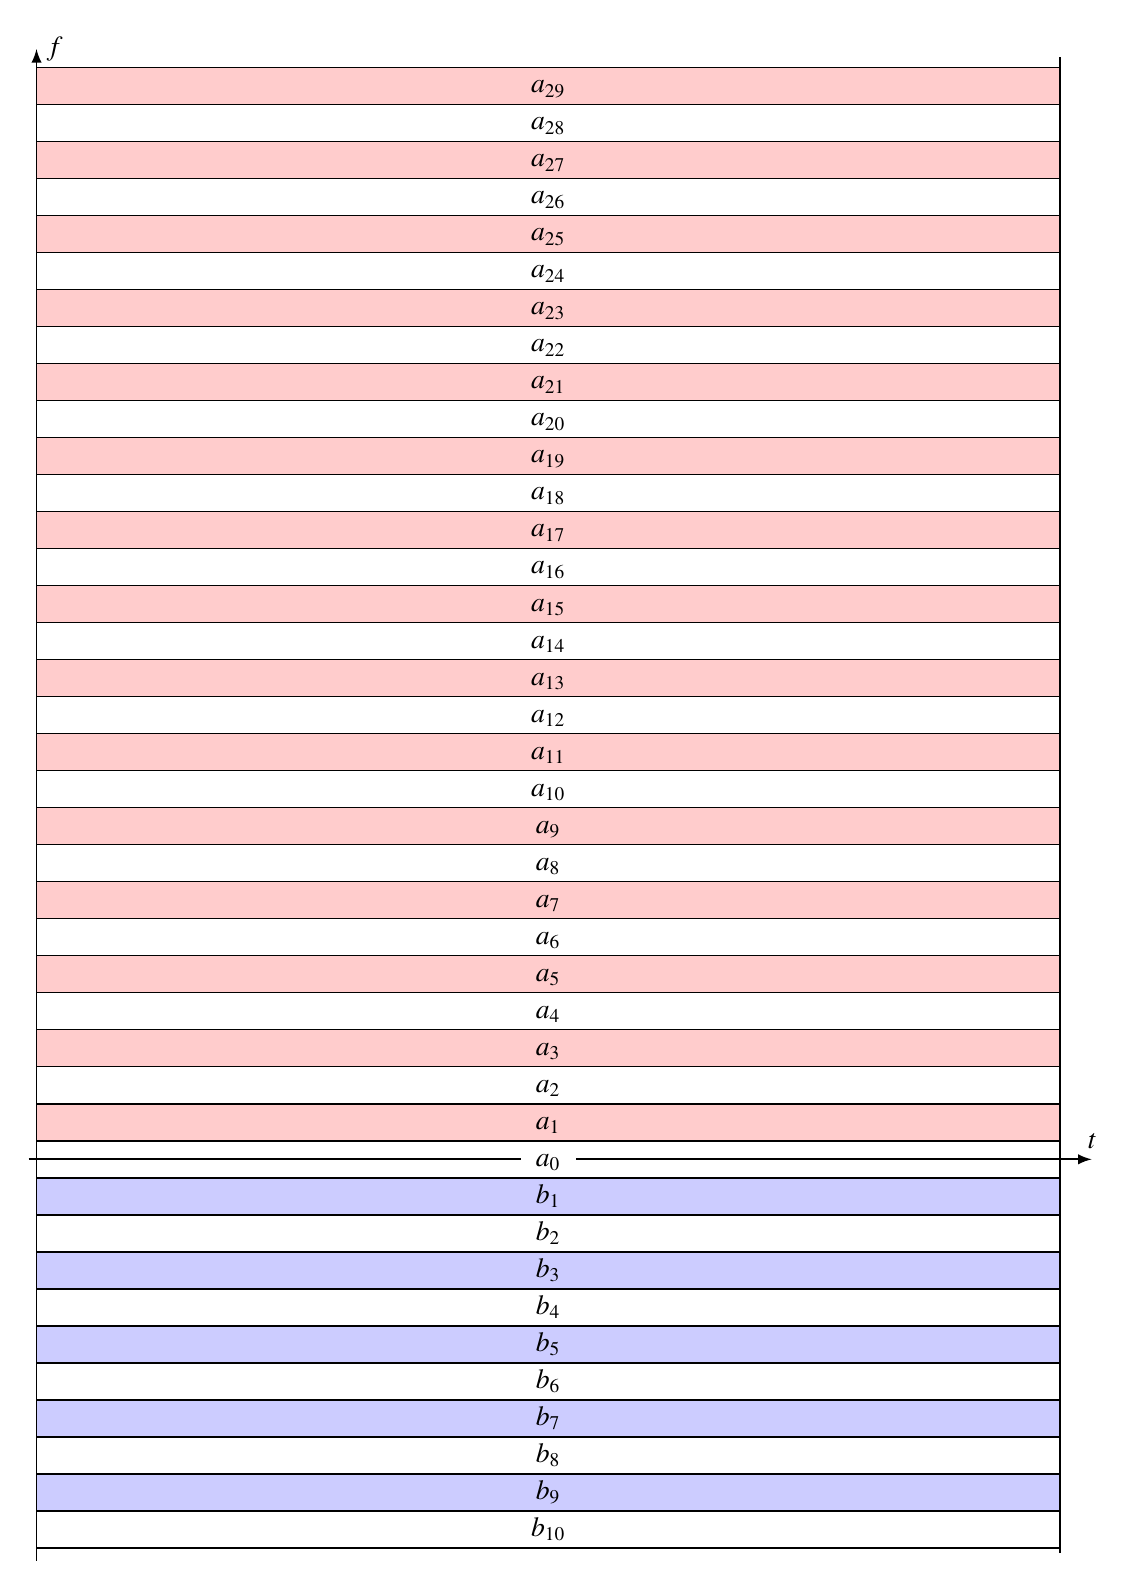
\begin{tikzpicture}[>=latex]

\def\h{0.47}
\def\w{13}

\pgfmathparse{14/\h}
\xdef\maxy{\pgfmathresult}
\pgfmathparse{-5/\h}
\xdef\miny{\pgfmathresult}

\foreach \y in {1,3,...,{\maxy}}{
	\fill[color=red!20] (0,{(\y-0.5)*\h})--({\w},{(\y-0.5)*\h})
		--({\w},{(\y+0.5)*\h})--(0,{(\y+0.5)*\h})--cycle;
}

\foreach \y in {1,...,{\maxy}}{
	\draw[line width=0.5pt] (0,{(\y+0.5)*\h})--({\w},{(\y+0.5)*\h});
	\node at ({\w/2},{\y*\h}) {$\mathstrut a_{\y}$};
}

\foreach \y in {1,3,...,{-\miny}}{
	\fill[color=blue!20] (0,{(-\y-0.5)*\h})--({\w},{(-\y-0.5)*\h})
		--({\w},{(-\y+0.5)*\h})--(0,{(-\y+0.5)*\h})--cycle;
}

\foreach \y in {1,2,...,{-\miny}}{
	\draw[line width=0.5pt] (0,{(-\y-0.5)*\h})--(\w,{(-\y-0.5)*\h});
	\node at ({\w/2},{-\y*\h}) {$\mathstrut b_{\y}$};
}

\draw[->,line width=0.7pt] (-0.1,0)--(13.4,0) coordinate[label={$t$}];
\draw[->,line width=0.7pt] (0,-5.1)--(0,14.1) coordinate[label={right:$f$}];
\draw[line width=0.5pt] (13,-5)--(13,14);

\fill[color=white] ({\w/2-0.35},{-\h/2})--({\w/2+0.35},{-\h/2})
	--({\w/2+0.35},{\h/2})--({\w/2-0.35},{\h/2})--cycle;
\node at ({\w/2},0) {$\mathstrut a_0$};

\draw[line width=0.7pt] (0,{\h/2})--({\w},{\h/2});
\draw[line width=0.7pt] (0,{-\h/2})--({\w},{-\h/2});

\end{tikzpicture}
\end{document}

